\documentclass[10pt,twocolumn]{article}
\usepackage[a4paper,margin=18mm]{geometry}
\usepackage[T1]{fontenc}
\usepackage{lmodern,amsmath,amssymb,amsfonts,graphicx,booktabs,array,url}
\usepackage[numbers,sort&compress]{natbib}
\usepackage[hidelinks]{hyperref}
\setlength{\columnsep}{7mm}
\title{Minimum-Useful-Service Continuity: A Reproducible Synthetic Benchmark and Metric-Semantics Audit for Edge Devices}
\author{Edmund Gunn, Jr.\\gunnchOS Research\\\texttt{egunnjr@gunnchos.com}\\ORCID: \href{https://orcid.org/0009-0004-6546-2609}{0009-0004-6546-2609}}
\date{gunnchOS Research Exploratory Preprint --- v0.1\\Local candidate for scientific review, 13 October 2026\\Not peer reviewed. Not posted. Publication authorization: false.}
\begin{document}
\maketitle
\begin{abstract}

Useful service on an edge device can persist after a network disconnection, while a connected device can still fail to complete a task. Evaluating continuity therefore requires explicit workload semantics and a clear boundary between measured and simulated evidence. This article develops and audits a reproducible synthetic benchmark that separates a deterministic service-profile corpus from a seeded continuity generator. The corpus contains 21 stored snapshots across four device profiles; eight offline snapshots preserve declared local workloads, whereas an unsupported wearable coding workload fails. All four snapshots labeled degraded Wi-Fi remain in the connected state and receive the target label, exposing incomplete stress coverage. A separate generator uses 30 recorded seeds, four synthetic device classes, and 48 abstract steps per class. Mean task completion is 0.4273 with a 95 percent interval of 0.4117 to 0.4428; mean time above minimum useful service is 0.5915 with an interval of 0.5765 to 0.6065. These intervals describe simulation variability. A source-level audit shows that several secondary endpoints duplicate the useful-time outcome and that the recovery counter records outage entries. Analytic expectations explain the generator's class ordering through its configured priors. The contribution is a transparent benchmark and an evidence-semantics audit, with explicit limits on hardware, radio, human-experience, and transferability claims. Physical calibration and independent policy comparisons remain necessary before deployment conclusions.

\end{abstract}
\noindent\textbf{Keywords:} 
Benchmarking, edge computing, minimum useful service, reproducibility, service continuity, synthetic simulation.


\noindent\textbf{Evidence status.} Synthetic fixture and simulation audit. Experimental source: \texttt{1a5491bf}; preserved journal source: \texttt{951a91e}; repaired-verifier source: \texttt{6523d11}. Full revisions and file hashes accompany this candidate. Human scientific approval, originality verification and article-license approval remain pending.

\section{Introduction}
\label{sec:intro}
Service continuity concerns whether a person can continue the task they need during a disruption. A device may lose its bearer yet retain a cached lesson, document editor, or local development tool. Conversely, a connected bearer alone does not establish that an application meets its deadline, has the needed data, or fits the available compute and memory. IMT-2030 identifies service-oriented resilience and ubiquitous connectivity as important directions~\cite{itur_m2160}; versioned 5G service requirements already distinguish performance expectations among services~\cite{3gpp_ts22261}. These frameworks motivate an application-sensitive evaluation, but they do not validate the thresholds or priors used in a particular simulation.

For resource-constrained edge devices, a useful evaluation must preserve both network and workload state. This article asks a deliberately bounded question: \emph{what does the currently implemented continuity benchmark establish about declared local workload support and simulated useful-service occupancy, and which apparently stronger conclusions are unsupported?} The evidence is digital: a frozen Device OS service-profile corpus and a separate seeded generator in the 7GC Digital Twin repository. The term digital twin identifies the repository and its research trajectory; the evaluated generator has no live physical counterpart or calibrated radio model.

The study makes three contributions. First, it formalizes and reproduces a four-level classification over 21 stored profile snapshots, including an explicit unsupported workload and the distinction between a scenario name and the state actually exercised. Second, it documents a 30-seed generator at the level of its random draws, synthetic class priors, and statistical unit, allowing exact reproduction and analytic interpretation of its two primary outcomes. Third, it audits the dependency structure and meaning of secondary metrics, identifies an outage-entry counter mislabeled as recovery, and states a prospective path to physical validation. These contributions concern benchmark semantics and reproducibility; they establish neither a new optimal controller nor a performance improvement over published systems.

The Gary flagship scenario supplies named disruption contexts such as neighborhood outages and congested school connectivity. It is an authored research scenario, rather than an operating community network. Five context names map to stored bearer labels. That mapping supplies a transparent scenario vocabulary, but does not model storm propagation, neighborhood infrastructure, payment transaction integrity, or RF interference. The analysis retains unfavorable and inconclusive findings instead of treating successful execution as evidence of general resilience.

The remainder distinguishes prior work, the two evidence paths, experimental versioning, reproduced outcomes, and threats to validity. A separate author-review supplement records exact hashes, commands, a data dictionary, citation checks, and claims requiring future evidence.

\subsection{Research Questions and Evidence Targets}
The first question asks which declared workload and connection-state combinations the stored classifier distinguishes, and which failure states its corpus leaves untested. The second asks which primary generator outcomes and metric relationships can be exactly reconstructed from its frozen seed specification. These are questions about this implementation and its evidence semantics. Neither question asks whether a measured device or network achieves a validated application threshold, nor whether a controller improves service over an executed competing policy.

\section{Related Work and Novelty Boundaries}
\label{sec:related}
\subsection{Resilience and Application Semantics}
Sterbenz et al.~\cite{sterbenz2010} define network resilience in terms of maintaining acceptable service despite faults and challenges, and distinguish operational network state from service state. Their multilevel framework and service-state analysis predate this benchmark. The minimum-useful vocabulary here is a small executable instance of an established service-sensitive idea, rather than a claim to have originated that idea. The contribution lies in exposing what this particular corpus exercises and in reconciling its numerical reporting with the code.

Edge computing can provide nearby processing and a fallback when remote cloud service is unavailable~\cite{satyanarayanan2017}. This supports the architectural motivation for local continuity, but local execution does not automatically preserve every workload. A local copy must contain the needed content, application, credentials, and adequate resources. The stored profiles encode only a declared coverage flag; they do not establish those conditions through physical execution.

\subsection{Benchmarking and Physical Anchoring}
EdgeDroid~\cite{olguin2019} records sensory traces, replays them through application task models, and collects pipeline timing from real client and cloudlet systems. Its workload-conditioned benchmarking is a close methodological comparator. The present corpus uses labeled snapshots and Bernoulli outcomes, without trace playback or execution of application code. It therefore cannot replace that kind of application measurement. A prospective extension could associate each continuity label with a trace-defined task, while preserving unsupported workloads as failures rather than changing the workload after the outage.

Fuller et al.~\cite{fuller2020} discuss digital-twin definitions, data requirements, and common confusion between twins and other digital representations. Contemporary work by Li et al.~\cite{li2025} proposes a native network digital-twin architecture and reports a comparison with real network testing for a signaling-storm use case. The abstract and official publication metadata of that article were inspected; its detailed experimental methodology was not available for full-text audit in this package. Its reported physical comparison nevertheless illustrates the evidence boundary absent here. We do not reproduce or compare numerically against its system.

\subsection{Claimed Increment}
Table~\ref{tab:novelty} positions the evidence relative to the inspected literature. The novelty claim is intentionally modest: a reproducible profile corpus alongside an explicit audit of synthetic endpoint semantics. Four-state classification, offline fallback, and digital-twin evaluation are established concepts. No exhaustive priority claim is made. The current study may remain too narrow for a research journal unless reviewers judge the semantic failures and reproducibility contribution sufficiently general or additional validation establishes that generality.

\begin{table*}[t]
\centering\caption{Contribution boundaries against closely related primary literature. These are methodological comparisons, not executed performance baselines.}\label{tab:novelty}
\small\begin{tabular}{p{0.19\textwidth}p{0.34\textwidth}p{0.38\textwidth}}\toprule
Source & Established contribution & Increment and boundary of this study \\\midrule
Sterbenz et al.~\cite{sterbenz2010} & Acceptable service under challenges; operational and service states & Executable small corpus and metric audit; no new general theory of resilience \\
Satyanarayanan~\cite{satyanarayanan2017} & Edge proximity and local fallback during cloud disruption & Workload support flags expose failure; no measured edge or cloud comparison \\
EdgeDroid~\cite{olguin2019} & Trace replay, task models, and measured application timing & Snapshot semantics and synthetic occupancy; no claim of equivalent workload realism \\
Fuller et al.~\cite{fuller2020} & Twin definitions, enabling technologies, and data-quality challenges & Clear physical-calibration boundary; no sensor-synchronized twin \\
Li et al.~\cite{li2025} & Native network twin with reported real-network comparison & Reproducibility audit only; no equivalent network-validation evidence \\
\bottomrule\end{tabular}
\end{table*}

\section{System Model and Implemented Methods}
\label{sec:method}
\subsection{Two Distinct Evidence Paths}
The benchmark has two paths (Fig.~\ref{fig:architecture}). The first reclassifies stored service-profile snapshots and applies a context-name mapping. The second produces seeded abstract timelines from synthetic class priors. They share outcome terminology, but neither path supplies the other's observations. In particular, the timeline does not derive its Bernoulli probabilities from the profile corpus, and its class names differ from the profile names. This distinction prevents an apparent combined validation from two artifacts that were never coupled.

\begin{figure}[t]
\centering
\fbox{\begin{minipage}{0.91\columnwidth}\small
\textbf{Path A: semantic corpus}\par
Frozen profiles + workload coverage $\longrightarrow$\par
State classification $\longrightarrow$ 21 labels\par
Authored context map $\longrightarrow$ 20 overlay rows\medskip\par
\textbf{Path B: stochastic generator}\par
Seed + four synthetic priors $\longrightarrow$\par
48 abstract steps per class $\longrightarrow$ $C_s,\tau_s$\par
30 seed means $\longrightarrow$ Student-$t$ intervals\medskip\par
\textbf{Audit layer}\par
Frozen hashes, source parity, metric dependencies,\par
post hoc analytic expectations and limitations
\end{minipage}}
\caption{Implemented evidence flow. No live sensors, channel calibration, workload execution, or policy optimizer connects the two paths.}\label{fig:architecture}
\end{figure}

\subsection{Profile-Based Minimum Useful Service}
Let $o$ be the stored orchestrator state and $F_{c,w}$ a Boolean declaration that profile $c$ supports workload $w$ offline. The implemented classifier is
\begin{equation}
L(o,F)=\begin{cases}
3,&o=\mathrm{connected},\\
2,&o\in\{\mathrm{degraded},\mathrm{transitioning}\},\\
1,&o=\mathrm{offline},\ F=1,\\
0,&\text{otherwise}.
\end{cases}\label{eq:classifier}
\end{equation}
The labels are target, degraded, minimum useful, and failed, respectively. The semantic acceptance predicate is $L\geq1$. These are ordered categories, not equally spaced utility scores. Averaging their numeric encodings would require a separate cardinal-utility assumption and is not done here.

For a hand check, an offline local-creation snapshot with declared workload support receives $L=1$, whereas an offline wearable coding request without support receives $L=0$. Changing only the stored state to connected yields $L=3$ for either request. This last case exposes a classifier limitation: capability and application success are not evaluated on the connected branch. These three evaluations illustrate the rule; they are not added observations.

The four profiles are desk, mobile/docked, local creation, and wearable. Each contains five common scenario snapshots; wearable includes a sixth unsupported coding request. Connected state receives the target label without checking measured latency, throughput, task correctness, or resource availability. Thus, \eqref{eq:classifier} operationalizes the repository's current \emph{declared} service threshold, not a user-validated threshold. It can expose an unsupported offline workload, but cannot detect a connected application failure if the stored state remains connected.

Five Gary context names map to common snapshots: neighborhood outage maps to jam/offline fallback; storm congestion, school bandwidth collapse, and library hotspot overload map to degraded Wi-Fi; payment-system unavailability maps to forced offline. The mapping is fixed in the versioned configuration. It is a lookup assumption, not a model of those events' physical causes or business consequences.

\subsection{Seeded Continuity Generator}
For each seed $s$, the simulator instantiates \texttt{random.Random(s)} and iterates over wearable, smartphone, laptop, and edge node, each for $T=48$ abstract steps. Let $a_c$, $q_c$, and $h_c$ denote class useful-service base probability, conditional task base probability, and stress sensitivity. Table~\ref{tab:priors} gives their exact values. At each step the code draws stress $S\sim U(0,1)$ and demand $D\sim U(1,50)$, then samples
\begin{align}
M_{sct}&\sim\mathrm{Bernoulli}\big[a_c(1-0.35h_cS)\big],\label{eq:useful}\\
Y_{sct}&=M_{sct}B_{sct},\label{eq:task}\\
B_{sct}&\sim\mathrm{Bernoulli}\big[q_c(1-0.2S)\big].\notag
\end{align}
The task draw is performed only if $M_{sct}=1$, exactly as in the implementation. Stress and Bernoulli draws use a pseudorandom stream; the displayed probability model describes their intended sampling semantics. All configured probabilities remain within $[0,1]$.

\begin{table}[t]\centering\caption{Synthetic timeline priors. Values are authored assumptions, not calibrated device measurements.}\label{tab:priors}\small
\begin{tabular}{lrrr}\toprule
Class & $a_c$ & $q_c$ & $h_c$\\\midrule
Wearable & 0.45 & 0.55 & 1.35\\
Smartphone & 0.72 & 0.78 & 1.00\\
Laptop & 0.80 & 0.85 & 0.85\\
Edge node & 0.88 & 0.90 & 0.70\\\bottomrule
\end{tabular}\end{table}

Useful occupancy and task completion for a class and seed are
\begin{equation}
\tau_{sc}=\frac1T\sum_{t=1}^{T}M_{sct},\qquad
C_{sc}=\frac1T\sum_{t=1}^{T}Y_{sct}.\label{eq:outcomes}
\end{equation}
The primary seed means weight all four classes equally: $\tau_s=\frac14\sum_c\tau_{sc}$ and $C_s=\frac14\sum_c C_{sc}$. Each step represents one synthetic task opportunity; it has no assigned number of seconds. Consequently, useful time is a fraction of equally weighted abstract steps, and completion is a synthetic success fraction rather than a measured jobs-per-second rate. There are 5,760 class-step outcomes across the 30 seeds, but the statistical sample size is 30 seed means.

Demand does not enter \eqref{eq:useful} or \eqref{eq:task}. It only contributes to the energy proxy. There is no queue, battery state, memory constraint, congestion feedback, traffic scheduler, radio channel, or admission-control decision in this generator. Resource constraint is represented indirectly by class-specific probabilities. A class ordering in the results therefore does not demonstrate a device performance ordering under equal physical workloads.

\subsection{Reporting Algorithm and Numerical Conventions}
The implementation loads the frozen bundle, rederives all stored labels, constructs the context overlay, generates a timeline for each recorded seed, and reports primary and secondary summaries. These steps are deterministic for the source, configuration, and Python random generator used. Reproduction must preserve class order and conditional draw behavior: consuming an extra random number, even for an unused task draw, changes subsequent samples.

Class fractions and seed aggregates are rounded to six decimals before the stored report computes across-seed summaries. The manuscript reports four decimals. The analytic model applies to the unrounded fractions. The maximum rounding discrepancy between an unrounded overall seed fraction and its stored value is at most $10^{-6}$, combining class and aggregate rounding. The statistical audit independently recalculates the stored means and intervals; it does not silently replace historical values with unrounded recalculations.

\section{Experimental Design and Reproducibility}
\label{sec:design}
\subsection{Protocol Versions and Provenance}
The current experiment uses seeds $1,2,\ldots,30$ and the configuration \texttt{rq1\_gary\_flagship\_profiles.yaml}. The evaluated source revision is \texttt{1a5491bf}\allowbreak\texttt{9261f77a}\allowbreak\texttt{75cc0fa7}\allowbreak\texttt{edbb5f25}\allowbreak\texttt{b425c7aa}. The protocol mirror in \texttt{paper/artifacts} is retained unchanged. Earlier source revision \texttt{376b6d67}\allowbreak\texttt{3ff6aaf1}\allowbreak\texttt{d60b5a73}\allowbreak\texttt{589f26d4}\allowbreak\texttt{9b46dbed} configured four seeds, $1,2,7,42$, for the original fixture and site-reporting path. Revision \texttt{b8c84e46}\allowbreak\texttt{5fc89e3e}\allowbreak\texttt{14915a1f}\allowbreak\texttt{30ff8491}\allowbreak\texttt{645f884a} introduced seeded statistical reporting; revision \texttt{dd0a7b07}\allowbreak\texttt{38f9e4e6}\allowbreak\texttt{5830ea23}\allowbreak\texttt{97fb4438}\allowbreak\texttt{e255d5b0} expanded the list to 30 and corrected statistical helpers.

Those revisions are distinct development stages. The earlier manuscript's four-seed language does not describe the current statistical results. Seed 42 is absent from the current list. The configuration is frozen in Git, but its history alone does not establish independent preregistration before analysis. The article therefore describes a versioned, specified seed list at the evaluated revision, and labels the analytic and semantic audits as post hoc. Historical prose and files remain recoverable separately.

The profile bundle's declared content digest is \texttt{ef5323a1}\allowbreak\texttt{607bf880}\allowbreak\texttt{31fb2093}\allowbreak\texttt{75325e39}\allowbreak\texttt{35049651}\allowbreak\texttt{346fcc13}\allowbreak\texttt{8f022b1a}\allowbreak\texttt{ba9c0083}; its full-file SHA-256 is \texttt{98f3a4e5}\allowbreak\texttt{bd76a1bd}\allowbreak\texttt{203af1a4}\allowbreak\texttt{797acc3b}\allowbreak\texttt{0041369e}\allowbreak\texttt{b8798454}\allowbreak\texttt{62b3a231}\allowbreak\texttt{ece6e46a}. These distinguish the recorded content identity from the file-byte checksum. The provenance file names the frozen supervisor-ready Device OS artifact as its source. It does not supply a source Git revision for that external bundle; that upstream identity remains a provenance limitation.

\subsection{Statistical Unit and Estimation}
For primary outcome $X_s\in\{C_s,\tau_s\}$, the report computes
\begin{equation}
\bar X=\frac1n\sum_s X_s,\quad
s_X^2=\frac1{n-1}\sum_s(X_s-\bar X)^2,\label{eq:stats}
\end{equation}
with $n=30$, and the two-sided interval
\begin{equation}
\bar X\ \pm\ t_{0.975,29}\frac{s_X}{\sqrt{30}},\qquad
 t_{0.975,29}=2.0452296421.\label{eq:ci}
\end{equation}
The source's tabulated critical value was independently checked using SciPy. The intervals characterize variation of seed means under this generator. They do not include parameter uncertainty, measurement error, bias in the offline coverage declarations, or uncertainty about a real population. Treating 5,760 class-step observations as independent experimental replicates would understate the uncertainty at the chosen seed level.

No competing controller is executed, and the report's paired-baseline and effect-size fields are null. Therefore no paired significance test, controller effect size, or causal superiority claim is reported. Per-class intervals are descriptive and unadjusted for simultaneous inference. The deterministic 21-snapshot corpus is an exhaustive enumeration of this stored bundle, not a random sample from a workload population; its counts receive no inferential confidence intervals.

\subsection{Reproduction and Secondary Analyses}
The recovered digital reproduction completed \texttt{make paper-reproduce}; its reproduction-stage tests passed 17 checks, and the focused profile/statistical tests passed 27. A derived reporting script verifies exact equality of the current per-seed, primary, secondary, and per-class summaries against the source revision's committed statistical report. Independent SciPy calculations reproduce the primary means, sample deviations, and intervals. These automated checks verify implementation and artifact parity; independent human replication remains pending.

The post hoc analyses consist of source inspection, closed-form expectations for the fixed generator, and a semantic comparator that assigns failure to every offline snapshot. The comparator is a classification-rule contrast, not an executed cloud-only controller or an offline-disabled physical system. No new simulation sweep, ablation campaign, hardware run, or parameter-fitting study was added during manuscript preparation. The package includes all figure sources, output hashes, environment records, and commands.

\subsection{Integrity and Provenance Checks}
The engine's \texttt{digest\_match} flag compares the bundle's stored content-digest identifier with the stored provenance identifier; it does not recompute a semantic digest over the bundle. The independent audit instead checks the actual file-byte SHA-256 against the retained provenance and exact frozen Git bytes. This verifies this archived file's identity, not the upstream production process or its physical truth. The repaired verifier compares all scientific values and stable provenance semantics exactly, while preserving and validating variable producer commit, timezone-bearing generation time, output locations and their dependent checksums separately. Whole-payload byte equality is not claimed. Deliberately altering a scientific value still fails after its checksum is recomputed.

\section{Reproduced Results}
\label{sec:results}
\subsection{Profile Corpus and Failure Coverage}
All 21 stored labels match the rederived classifier, and the recorded content digest matches provenance. Table~\ref{tab:fixture} and Fig.~\ref{fig:fixture} show 12 target, eight minimum-useful, zero degraded, and one failed snapshot. The failure is the wearable profile's explicit unsupported offline coding request. The result follows directly from an offline state with $F_{c,w}=0$ in \eqref{eq:classifier}; it does not measure failed compilation or execution on a wearable.
\begin{table}[t]
\centering
\caption{Exhaustive counts in the 21 stored profile snapshots. No degraded or transitioning state is exercised.}
\label{tab:fixture}
\par\smallskip
\small
\begin{tabular}{lrrrr}
\toprule
Profile & Target & Degraded & Useful & Failed \\
\midrule
desk & 3 & 0 & 2 & 0 \\
mobile/docked & 3 & 0 & 2 & 0 \\
local/creation & 3 & 0 & 2 & 0 \\
wearable & 3 & 0 & 2 & 1 \\
\bottomrule
\end{tabular}
\end{table}


The three other profiles each have three target and two minimum-useful rows. The wearable has the same common five rows plus the unsupported request. This asymmetry prevents interpreting raw failure counts as fair comparative device reliability. The corpus deliberately probes a missing wearable capability while omitting analogous unsupported tasks for the other profiles.

\begin{figure*}[t]\centering
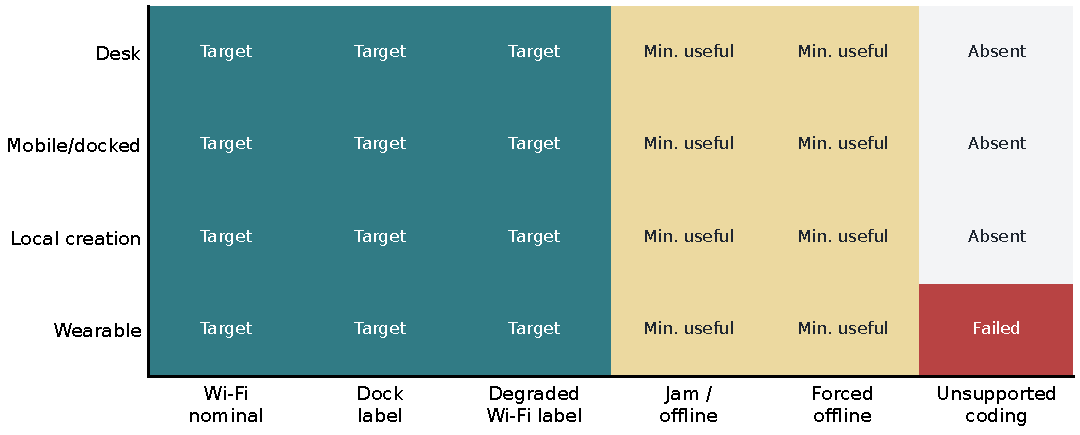
\includegraphics[width=0.91\textwidth]{figures/owner_fixture_matrix.pdf}
\caption{The 21 frozen snapshots. Absent cells are untested combinations. All four degraded-Wi-Fi labels retain connected state and therefore receive target. No snapshot exercises degraded or transitioning state.}\label{fig:fixture}
\end{figure*}

All four scenarios named degraded Wi-Fi receive target because their stored orchestrator state is connected. Hence the scenario label does not establish a degraded-service observation. The zero degraded count exposes a coverage gap in the fixture, even though the classifier has a degraded branch. The 20 Gary overlay rows contain no below-minimum-useful outcome because the context mapping selects declared supported workloads. This is a property of that mapping and workload selection, not evidence that all real disruptions preserve useful service.

The post hoc connected-only semantic comparator labels all nine offline rows failed. The benchmark instead identifies eight as minimum useful and one as failed. The eight reclassifications show precisely what the coverage declaration adds to a connectivity-only label. They do not quantify a policy improvement: no fallback action, application execution, or user benefit was measured in this comparison.

\subsection{Thirty-Seed Primary Outcomes}
Table~\ref{tab:primary} gives the reproduced overall outcomes. Task completion is 0.427257 with sample standard deviation 0.041610; useful occupancy is 0.591493 with standard deviation 0.040243. Their 95\% seed-level intervals are [0.411720,0.442795] and [0.576466,0.606520], respectively. Completion is bounded by useful occupancy at every class and step by \eqref{eq:task}; the lower completion mean reflects the conditional task-success gate.
\begin{table}[t]
\centering
\caption{Frozen seeded timeline outcomes; 95\% Student-$t$ intervals over 30 seed means.}
\label{tab:primary}
\par\smallskip
\small
\begin{tabular}{lrrl}
\toprule
Outcome & Mean & SD & 95\% CI \\
\midrule
Completion $C$ & 0.4273 & 0.0416 & [0.4117, 0.4428] \\
Useful time $\tau$ & 0.5915 & 0.0402 & [0.5765, 0.6065] \\
\bottomrule
\end{tabular}
\end{table}


\begin{figure}[t]\centering
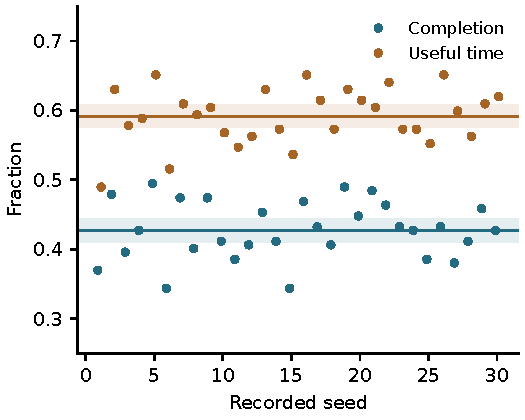
\includegraphics[width=\columnwidth]{figures/owner_seed_outcomes.pdf}
\caption{All 30 recorded seed means. Lines show means and shaded bands show their 95\% Student-$t$ intervals. These are intervals for generator means, not prediction bands for real deployments.}\label{fig:seeds}
\end{figure}

The observed overall completion range is approximately 0.344 to 0.495 and the useful-occupancy range 0.490 to 0.651 (Fig.~\ref{fig:seeds}). The intervals use all recorded seeds; none were removed based on outcome. Changing the seed set, step count, or prior values creates a different experiment and must be versioned separately.

\subsection{Class Priors and Analytic Interpretation}
The four timeline classes differ from the four profile categories. Table~\ref{tab:classes} therefore summarizes the stochastic classes independently. Wearable completion and useful occupancy are about 0.171 and 0.348; edge-node values are 0.628 and 0.786. The ordering is consistent with the authored probabilities and stress sensitivities.
\begin{table}[t]
\centering
\caption{Timeline classes have synthetic resilience priors; intervals describe the generator, not measured hardware.}
\label{tab:classes}
\par\smallskip
\footnotesize
\setlength{\tabcolsep}{3pt}
\begin{tabular}{lrlrl}
\toprule
Class & $C$ & 95\% CI & $\tau$ & 95\% CI \\
\midrule
wearable & 0.171 & [0.148, 0.193] & 0.348 & [0.320, 0.376] \\
smartphone & 0.392 & [0.365, 0.419] & 0.569 & [0.543, 0.594] \\
laptop & 0.519 & [0.491, 0.546] & 0.663 & [0.634, 0.692] \\
edge node & 0.628 & [0.596, 0.660] & 0.786 & [0.761, 0.811] \\
\bottomrule
\end{tabular}
\end{table}


For $b_c=0.35h_c$, the unrounded model yields the post hoc expectations
\begin{align}
\mathbb E[\tau_c]&=a_c(1-b_c/2),\label{eq:exp_tau}\\
\mathbb E[C_c]&=a_cq_c\left[1-\frac{b_c+0.2}{2}+\frac{0.2b_c}{3}\right].\label{eq:exp_c}
\end{align}
These integrate \eqref{eq:useful} and \eqref{eq:task} over uniform stress. Expected completion values for wearable, smartphone, laptop, and edge node are 0.1721, 0.4203, 0.5243, and 0.6287; expected useful fractions are 0.3437, 0.5940, 0.6810, and 0.7722. Fig.~\ref{fig:classes} places these values beside the simulation estimates. The smartphone completion expectation lies just above its descriptive interval; the study has not performed a formal goodness-of-fit test or simultaneous-coverage assessment. The analytic calculation is a model interpretation, not an additional independent experiment.

\begin{figure}[t]\centering
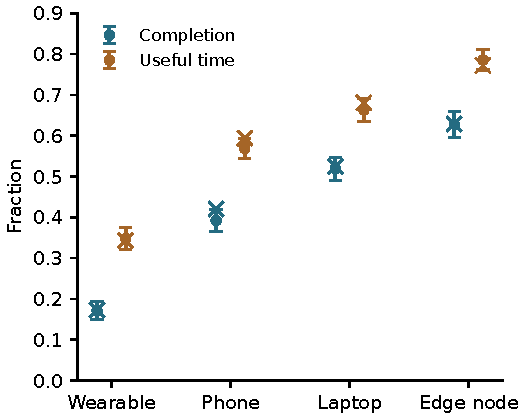
\includegraphics[width=\columnwidth]{figures/owner_class_outcomes.pdf}
\caption{Class means and descriptive 95\% intervals. Crosses mark post hoc analytic expectations. The class ordering reflects configured priors, with no calibrated hardware ranking implied.}\label{fig:classes}
\end{figure}

\subsection{Secondary Endpoint Audit}
The source defines reliability equal to useful occupancy. Outage fraction, QoE-violation fraction, and packet-loss proxy each equal its complement; throughput proxy is five times useful occupancy; compute-completion-time proxy is $T(1.2-0.4C)$. The identities hold up to reporting precision (Table~\ref{tab:metrics}). These fields are retained in machine-readable outputs for historical compatibility, but do not constitute independent validation of reliability, packet loss, quality of experience, throughput, or compute performance.

The field \texttt{recovery\_event\_count} increments when a failed step follows a non-outage step, including entry into an initial outage. It counts outage episodes entered, rather than successful recoveries. It is excluded from the aggregated secondary-key list. No recovery duration, restored-task fraction, or completed-recovery count is reported as an empirical result.

\begin{table}[t]\centering\caption{Metric meanings established by source inspection; historical field names are preserved in artifacts.}\label{tab:metrics}\small
\begin{tabular}{p{0.39\columnwidth}p{0.49\columnwidth}}\toprule
Reported field & Implemented definition and interpretation\\\midrule
Reliability & $\tau$; duplicate primary endpoint\\
Outage / QoE violation / packet-loss proxy & $1-\tau$; three duplicate complements\\
Throughput proxy & $5\tau$; arbitrary Mbps scaling\\
Compute completion proxy & $T(1.2-0.4C)$; synthetic transform\\
Recovery-event count & Number of outage entries; no completion test\\
Latency / jitter & Affine stress proxy / consecutive absolute differences\\
Energy proxy & Demand-weighted synthetic sum; no battery model\\\bottomrule
\end{tabular}\end{table}

\section{Discussion and Validation Implications}
\label{sec:discussion}
\subsection{What the Benchmark Establishes}
The fixture makes a useful logical distinction: network loss and declared workload loss need not coincide. The unsupported wearable request provides a counterexample to universal local continuity within the corpus. The degraded-Wi-Fi snapshots provide a second counterexample, showing that a stress name alone cannot demonstrate degraded behavior. Together, these findings support a benchmark-design lesson: report the exercised states and unsupported workload combinations, as well as successful labels.

The seeded experiment adds reproducible variability and explicit completion and occupancy outcomes. It does not validate the classifier, because it samples a separate minimum-useful Boolean from class priors. Its outcomes can be analytically understood from those priors. Increasing the seed count reduces Monte Carlo uncertainty about the chosen model; it does not reduce uncertainty about whether that model represents a real device or workload. The relatively narrow intervals should be interpreted in that light.

The endpoint audit also changes the interpretation of broad metric panels. Reporting reliability, loss, outage, and QoE together can suggest several confirming observations even when the code computes each from the same Boolean sequence. An audit should trace each metric to its generating observations and retain distinct measurements only where their relationship is explicit. This study exposes the redundancy rather than assigning a composite score or selecting the most favorable endpoint.

\subsection{Missing Comparisons and Prospective Study Design}
The current repository does not execute terrestrial-only, cloud-only, local-only, or oracle continuity controllers in this experiment. Literature comparisons in Section~\ref{sec:related} are conceptual. A fair prospective study would give each executed controller the same workload arrivals, sensor information, device budgets, outage traces, switching costs, and recovery opportunities. If an oracle receives future information, it should be labeled an unattainable reference bound and analyzed separately. These conditions are future design requirements, not guarantees established by the current code.

A physical study should define a minimum useful outcome per workload before collecting comparison data. For a cached lesson this may include readable content and saved progress; for coding it may include correct local execution of a named program; for payment it must address authorization and durable transaction semantics, so a generic offline-capability flag is insufficient. Numerical latency, deadline, accuracy, memory, energy, and data-freshness thresholds should be justified through task requirements or a separate user study. No such physical threshold study has been completed here.

A second prospective stage should run those workloads during controlled bearer loss, congestion, device resource pressure, and restoration, recording timestamps and task outcomes. It should compare classification against observed utility, including connected failures and false declarations of offline support. Calibration data and held-out validation traces must be separated. Bursty outages and correlated demand should replace independent stress only under a new versioned protocol. This would connect the current semantic corpus to a measured twin-state construction without retroactively changing the frozen benchmark.

\subsection{Relation to the Three-Paper Research Program}
This article provides workload semantics and an auditable reporting boundary. A separate cross-layer-control study asks how radio and orchestration decisions change modeled performance; a separate terrestrial/non-terrestrial study asks when fallback paths are beneficial or costly. Those decision problems require their own implemented controllers and experiments. Shared motivation or vocabulary does not prove independent scholarly novelty. Reuse of this corpus in either companion study must cite its exact version and must not count the same outcomes again as independent evidence.

The earlier physical-measurement roadmap and the later minimum-useful-service roadmap remain compatible as sequential research stages: this benchmark defines what should be observed, while field campaigns could determine whether its assumptions hold. Today the evidence supports the benchmark stage. It does not establish physical channel characterization, synchronized twin-state fidelity, operational 6G performance, or any university-affiliated research activity.

\subsection{Relationship to Companion Models}
The companion control study's dimensionless reliability--delay utility and categorical fidelity action are not this paper's declared workload classifier or Bernoulli useful-state generator. The companion TN--NTN study uses a configured 1 Mbps/500 ms path-qualification predicate, not the offline-coverage rule here. Shared continuity terminology and abstract steps do not make their outcomes interchangeable. The present corpus supplies no calibrated state-estimation accuracy, common controller observations, packet trace or power measurement for either companion. All three studies require separate scientific and originality review.

\section{Limitations and Threats to Validity}
\label{sec:limitations}
\textbf{Construct validity.} The profile threshold is a state-and-coverage rule. It lacks independent workload execution, task correctness, deadlines, and human judgments. Connected states always receive target, and degraded states always remain above the semantic threshold. Their suitability for a specific workload is untested. Timeline completion is a Bernoulli success event; a task does not have a measured duration or application-specific resource footprint.

\textbf{Internal validity.} The timeline classes and profile classes are different taxonomies. Their association is not calibrated, so they cannot be fused into one device experiment. The generator consumes one pseudorandom stream sequentially, with conditional task draws. Reproduction requires preserving the implementation order. Source-level identities make several secondary metrics redundant; an increase in one proxy is not corroboration from a second physical endpoint. Digest matching verifies consistency of stored identifiers, while the full-file hash records bytes; neither validates physical truth.

\textbf{External validity.} Four authored profile categories and 21 snapshots cannot represent all edge workloads, hardware, networks, or communities. The corpus omits many unsupported-task combinations, and the overlay reuses the same snapshots under different disruption names. Zero failures in its 20 rows does not estimate population outage risk. Other named geographic scenarios contain authored profiles, constant radio stubs, or barrier-list composites rather than sampled community observations. We exclude those composites from continuity performance claims.

\textbf{Statistical validity.} Seed intervals omit uncertainty in $a_c,q_c,h_c$ and distributional assumptions. The 48-step horizon and independent stress are not real outage durations or correlated infrastructure failures. Per-class intervals are descriptive, with no adjustment for multiple comparisons. No paired baseline or performance hypothesis test was executed. Analytic expectations and semantic relabeling were developed after inspecting the implementation and are explicitly post hoc. The larger current seed list must not be attributed retroactively to the four-seed historical protocol.

\textbf{Numerical and physical interpretation.} Energy, latency, jitter, packet loss, and throughput fields use proxy equations rather than instrumented measurements. They cannot support battery-life, joule, millisecond, RF, carrier, or hardware superiority claims despite unit-like field names. The study includes no spectrum measurements, fading model, satellite terminal, university campaign, community deployment, or user study.

\textbf{Provenance and reproducibility.} The frozen external profile bundle lacks an upstream source commit in its provenance record. The local reproduction and independent calculations were AI-assisted and are not independent human sign-off. Package dependencies were recorded for the recovered environment; portability to other Python versions and architectures requires confirmation. The manuscript preserves these limitations rather than interpreting the automated test count as scientific validation.

\textbf{Publication suitability.} The methodological contribution remains small and its transferability unproven. An author-review package can be technically complete while peer-review suitability remains uncertain. Owner review should determine whether the metric audit and benchmark failure coverage justify journal submission now or whether the prospective physical and policy studies are needed first.

\section{Conclusion}
This study reproduces and audits a minimum-useful-service benchmark without exceeding its digital evidence. The 21-snapshot corpus distinguishes eight declared useful offline cases from one unsupported request, while revealing that the degraded-Wi-Fi labels never exercise degraded states. The separate 30-seed generator yields completion 0.4273 and useful occupancy 0.5915, with seed-level uncertainty verified independently. Its class ordering follows synthetic priors, several secondary endpoints repeat the same underlying outcomes, and its recovery counter measures outage entry. These findings make the package useful as a transparent benchmark and a test of reporting semantics. Establishing deployment relevance requires workload execution, physical calibration, measured recovery, and fair controller comparisons under a new protocol.


\section*{Acknowledgment and Author-Review Declarations}
\textbf{Author information:} Edmund Gunn, Jr.; gunnchOS Research; egunnjr@gunnchos.com; ORCID 0009-0004-6546-2609. Additional authors, if any, remain pending owner confirmation.

\textbf{AI assistance:} OpenAI ChatGPT/Codex tools~\cite{openai_codex} were used for substantive manuscript drafting and editing, literature and metadata investigation, source and claim auditing, statistical verification code, figure-generation code, and LaTeX packaging. Figures are programmatic renderings of frozen synthetic artifacts, rather than generated physical measurements. The abstract and Sections 1--8 contain AI-assisted prose; the equations, statistical checks, and programmatic figures also received AI assistance. The author must review and verify all text, citations, calculations, code, and illustrations before submission and remains responsible for the final work. The precise session and model inventory is supplied in the review package where known; no AI system is listed as a human author.

\textbf{Data and code:} The evaluated source revision, frozen synthetic profiles, protocol, recorded seeds, reproduced outputs, analysis scripts, and environment records are included in the separate bounded evidence archive. The repository is gunnchOS3k/7gc-digital-twin. A permanent reviewed public archive and its identifier remain pending release authorization. Repository software carries an MIT license; profile and new article rights require the checks listed in the package before redistribution.

\textbf{Funding, conflicts, contributions, and rights:} Final funding and sponsor statements, conflicts of interest, human author contributions, and intellectual-property declarations remain pending owner review. This draft does not assert absence of funding, conflicts, sponsors, or additional authors. No submission, acceptance, publisher endorsement, or university affiliation is claimed.

Human scientific approval, originality verification, article-license approval, and public-release authorization remain false for this local candidate. No University of Oulu enrollment, supervision, research-unit endorsement or funding is claimed. The synthetic outputs contain no field-measurement study; no institutional ethics clearance is inferred.

\bibliographystyle{plainnat}
\bibliography{references}
\end{document}
